\documentclass[aspectratio=169,11pt]{beamer}
\usepackage[spanish,es-nodecimaldot]{babel}
\usepackage{amsmath,booktabs,graphicx,tikz}
\usetikzlibrary{arrows.meta,positioning}

\definecolor{AzulNoche}{HTML}{071A2B}
\definecolor{Azul}{HTML}{1261A0}
\definecolor{Cian}{HTML}{20B8CD}
\definecolor{Dorado}{HTML}{E8B44F}
\definecolor{GrisClaro}{HTML}{EEF4F7}
\definecolor{Verde}{HTML}{198F75}
\definecolor{Rojo}{HTML}{C84A5B}

\setbeamercolor{normal text}{fg=AzulNoche,bg=white}
\setbeamercolor{structure}{fg=Azul}
\setbeamercolor{frametitle}{fg=white,bg=AzulNoche}
\setbeamercolor{title}{fg=white}
\setbeamercolor{subtitle}{fg=Cian}
\setbeamercolor{block title}{fg=white,bg=Azul}
\setbeamercolor{block body}{fg=AzulNoche,bg=GrisClaro}
\setbeamercolor{alerted text}{fg=Rojo}
\setbeamertemplate{navigation symbols}{}
\setbeamertemplate{itemize item}{\color{Cian}$\blacktriangleright$}
\setbeamertemplate{footline}{%
  \hfill\usebeamerfont{page number in head/foot}%
  \color{Azul}\insertframenumber\hspace{0.7em}\vspace{0.45em}}
\setbeamertemplate{frametitle}{%
  \nointerlineskip\begin{beamercolorbox}[sep=.55em,wd=\paperwidth]{frametitle}%
  \usebeamerfont{frametitle}\insertframetitle
  \end{beamercolorbox}}

\graphicspath{{../figures/}{./}}
\title{Clasificación de flores con VGG16}
\subtitle{Comparación de tres cabezales clasificadores}
\author{Guillermo Tinoco Ramos}
\date{}

\newcommand{\dato}[2]{%
\begin{beamercolorbox}[rounded=true,sep=.55em,center,wd=.95\linewidth]{block body}
{\color{Azul}\Large\bfseries #1}\par\smallskip
{\small #2}
\end{beamercolorbox}}

\begin{document}

% 1 — 0:40
\begin{frame}[plain]
\begin{tikzpicture}[remember picture,overlay]
\fill[AzulNoche] (current page.south west) rectangle (current page.north east);
\fill[Cian,opacity=.16] (current page.south west) rectangle ([xshift=4.6cm]current page.north west);
\foreach \x/\y in {1.0/1.0,1.8/2.2,2.6/1.4,3.4/2.8,1.2/4.3,2.3/5.3,3.5/4.7}{
  \fill[Cian,opacity=.7] ([xshift=\x cm,yshift=\y cm]current page.south west) circle (2.5pt);}
\end{tikzpicture}
\vspace{1.0cm}
\hspace{4.3cm}\begin{minipage}{.62\textwidth}
{\usebeamerfont{title}\color{white}\LARGE\bfseries Clasificación de flores con VGG16\par}
\vspace{.25cm}
{\color{Cian}\large Comparación de tres cabezales clasificadores\par}
\vspace{1.0cm}
{\color{white}\normalsize Guillermo Tinoco Ramos\par}
\vspace{.2cm}
{\color{white!70}\small Objetivo: medir si una mayor complejidad mejora la clasificación.}
\end{minipage}
\end{frame}

% 2 — 1:00
\begin{frame}{El problema y los datos}
\begin{columns}[T,onlytextwidth]
\column{.58\textwidth}
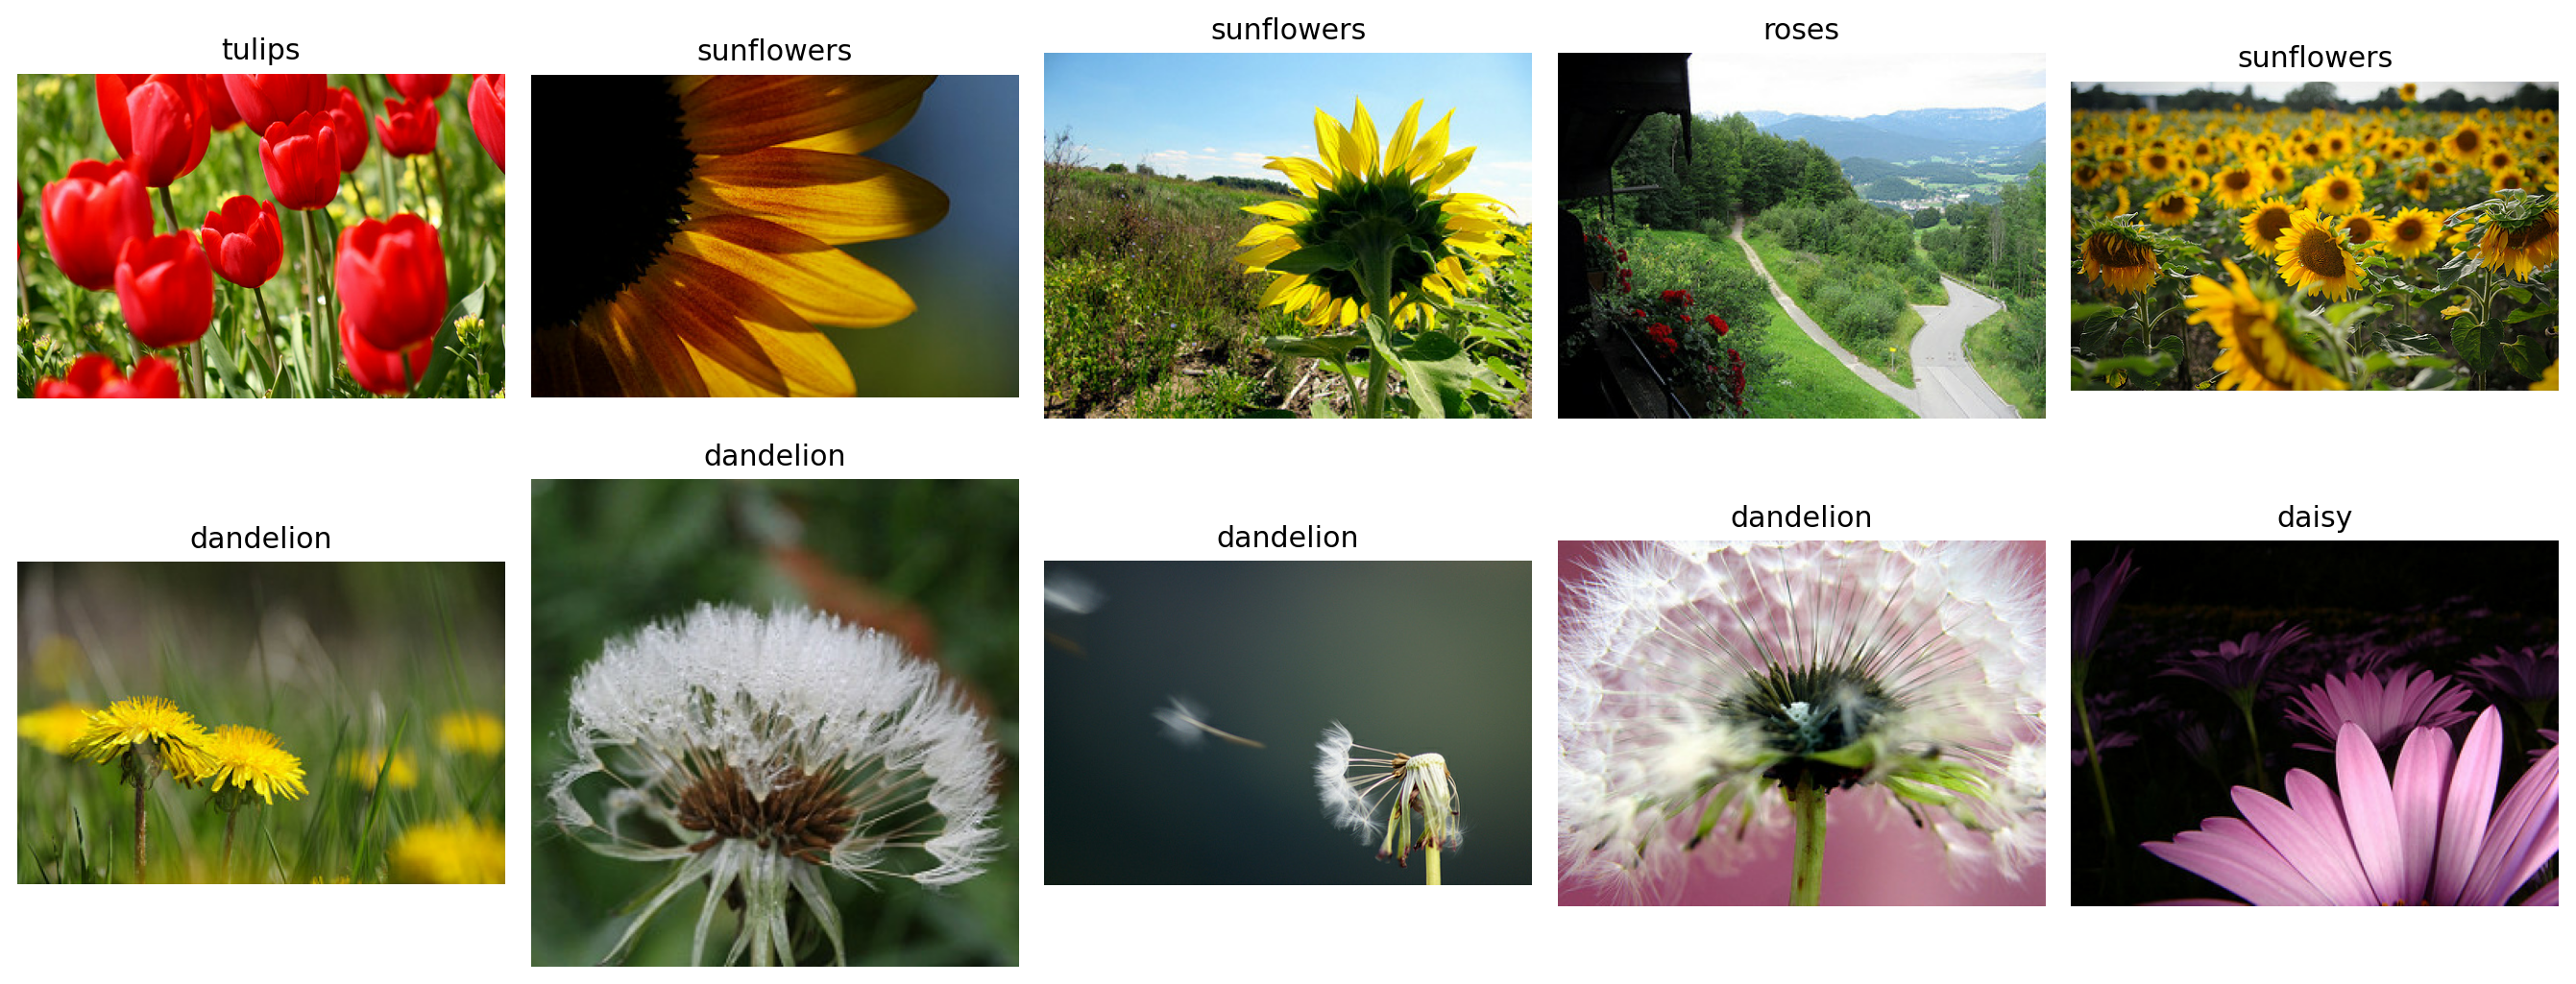
\includegraphics[width=\linewidth,height=.60\textheight,keepaspectratio]{mosaico_dataset.png}
\column{.38\textwidth}
\vspace{.15cm}
\dato{3,670}{imágenes RGB}
\vspace{.15cm}
\dato{5}{clases de flores}
\vspace{.15cm}
\dato{70 / 15 / 15}{partición estratificada: entrenamiento, validación y prueba}
\end{columns}
\end{frame}

% 3 — 1:20
\begin{frame}{Transfer learning: reutilizar antes que empezar de cero}
\centering
\resizebox{\textwidth}{!}{\begin{tikzpicture}[node distance=7mm,>=Latex,every node/.style={align=center,font=\small}]
\node[draw=Azul,rounded corners,fill=GrisClaro,minimum width=2.2cm,minimum height=1.1cm] (in) {Imagen\\$224\times224\times3$};
\node[draw=Azul,rounded corners,fill=Azul!12,right=of in,minimum width=3.2cm,minimum height=1.3cm] (vgg) {VGG16 + ImageNet\\\textbf{congelada}};
\node[draw=Verde,rounded corners,fill=Verde!12,right=of vgg,minimum width=2.2cm,minimum height=1.3cm] (maps) {$7\times7\times512$\\mapas};
\node[draw=Cian,rounded corners,fill=Cian!12,right=of maps,minimum width=3.2cm,minimum height=1.3cm] (gap) {Global Average\\Pooling};
\node[draw=Dorado,rounded corners,fill=Dorado!18,right=of gap,minimum width=2.0cm,minimum height=1.3cm] (vec) {512\\características};
\draw[->,thick,Azul] (in)--(vgg); \draw[->,thick,Azul] (vgg)--(maps);
\draw[->,thick,Azul] (maps)--(gap); \draw[->,thick,Azul] (gap)--(vec);
\end{tikzpicture}}
\vspace{.55cm}
\begin{columns}[T,onlytextwidth]
\column{.48\textwidth}
\begin{block}{?`Qué aporta VGG16?}
Filtros ya entrenados para reconocer bordes, texturas, formas y partes de objetos.
\end{block}
\column{.48\textwidth}
\begin{block}{?`Por qué no \texttt{Flatten}?}
Produciría 25,088 entradas y millones de pesos. El promedio global reduce costo y sobreajuste.
\end{block}
\end{columns}
\end{frame}

% 4 — 1:10
\begin{frame}{Una comparación controlada, no tres modelos arbitrarios}
\begin{columns}[T,onlytextwidth]
\column{.31\textwidth}
\begin{block}{A · mínimo}
\centering\Large\bfseries ?`VGG16 ya separa las clases?\par
\vspace{.35cm}\normalsize Frontera lineal
\end{block}
\column{.31\textwidth}
\begin{block}{B · intermedio}
\centering\Large\bfseries ?`Ayuda una combinación no lineal?\par
\vspace{.35cm}\normalsize 256 unidades ReLU
\end{block}
\column{.31\textwidth}
\begin{block}{C · profundo}
\centering\Large\bfseries ?`Más capacidad regularizada mejora?\par
\vspace{.35cm}\normalsize Dos capas + Dropout
\end{block}
\end{columns}
\vfill
\centering
\color{AzulNoche}\large\bfseries Mismos datos + misma VGG16 + mismo entrenamiento\\
\color{Cian}\normalsize Solo cambia el cabezal clasificador
\end{frame}

% 5 — 1:25
\begin{frame}{Arquitecturas: capacidad creciente}
\centering
\small
\begin{tabular}{@{}clrr@{}}
\toprule
\textbf{Modelo} & \textbf{Cabezal después de 512 características} & \textbf{Entrenables} & \textbf{vs. A}\\
\midrule
\color{Verde}\bfseries A & \texttt{Dense(5, softmax)} & \textbf{2,565} & $1\times$\\
\addlinespace
\color{Azul}\bfseries B & \texttt{Dense(256, relu)} $\rightarrow$ \texttt{Dense(5, softmax)} & 132,613 & $52\times$\\
\addlinespace
\color{Rojo}\bfseries C & \texttt{Dense(512, relu)} $\rightarrow$ \texttt{Dropout(0.5)} & 328,965 & $128\times$\\
& $\rightarrow$ \texttt{Dense(128, relu)} $\rightarrow$ \texttt{Dense(5, softmax)} &&\\
\bottomrule
\end{tabular}
\vspace{.55cm}
\begin{columns}[T,onlytextwidth]
\column{.48\textwidth}
\begin{block}{\texttt{Dense}}
Aprende nuevas combinaciones de las 512 características mediante pesos y sesgos.
\end{block}
\column{.48\textwidth}
\begin{block}{\texttt{Dropout}}
Desactiva activaciones al azar durante entrenamiento para reducir coadaptación.
\end{block}
\end{columns}
\end{frame}

% 6 — 0:40
\begin{frame}{Modelo A: VGG16 + clasificador lineal}
\centering
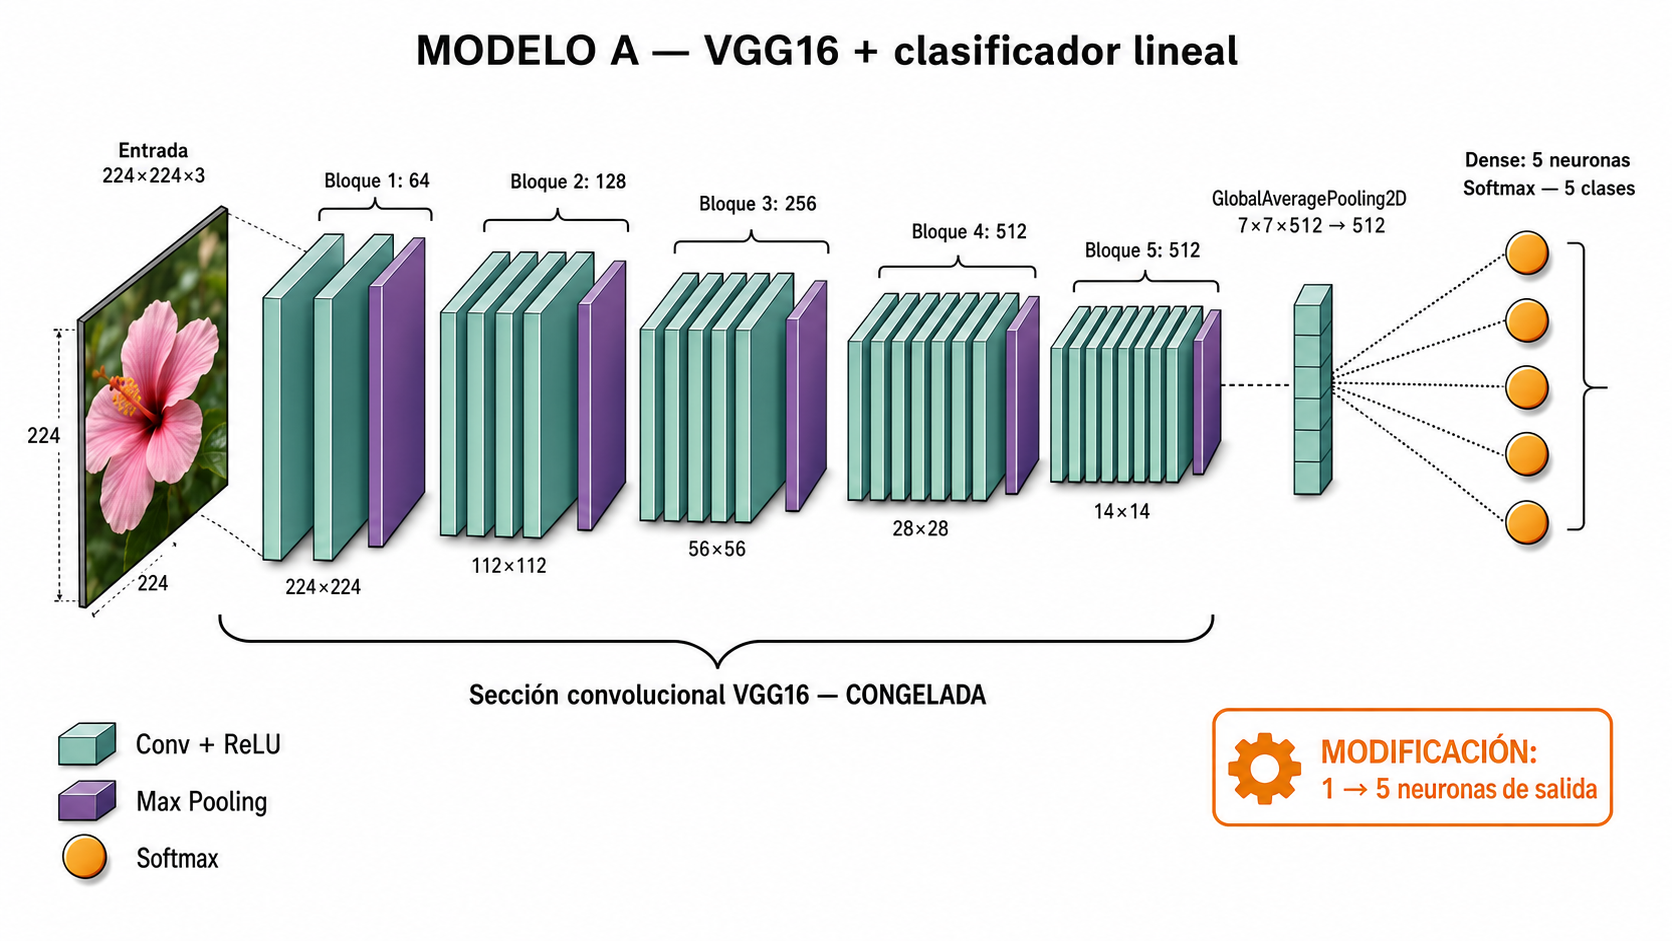
\includegraphics[width=.94\textwidth,height=.68\textheight,keepaspectratio]{arquitectura_modelo_A_visual.png}
\vspace{.08cm}
\begin{beamercolorbox}[rounded=true,sep=.35em,center,wd=.94\textwidth]{block body}
\scriptsize Los cinco bloques de VGG16 permanecen congelados; el vector de 512 características se conecta directamente con las cinco salidas \texttt{softmax}.
\end{beamercolorbox}
\end{frame}

% 7 — 0:40
\begin{frame}{Modelo B: una capa densa intermedia}
\centering
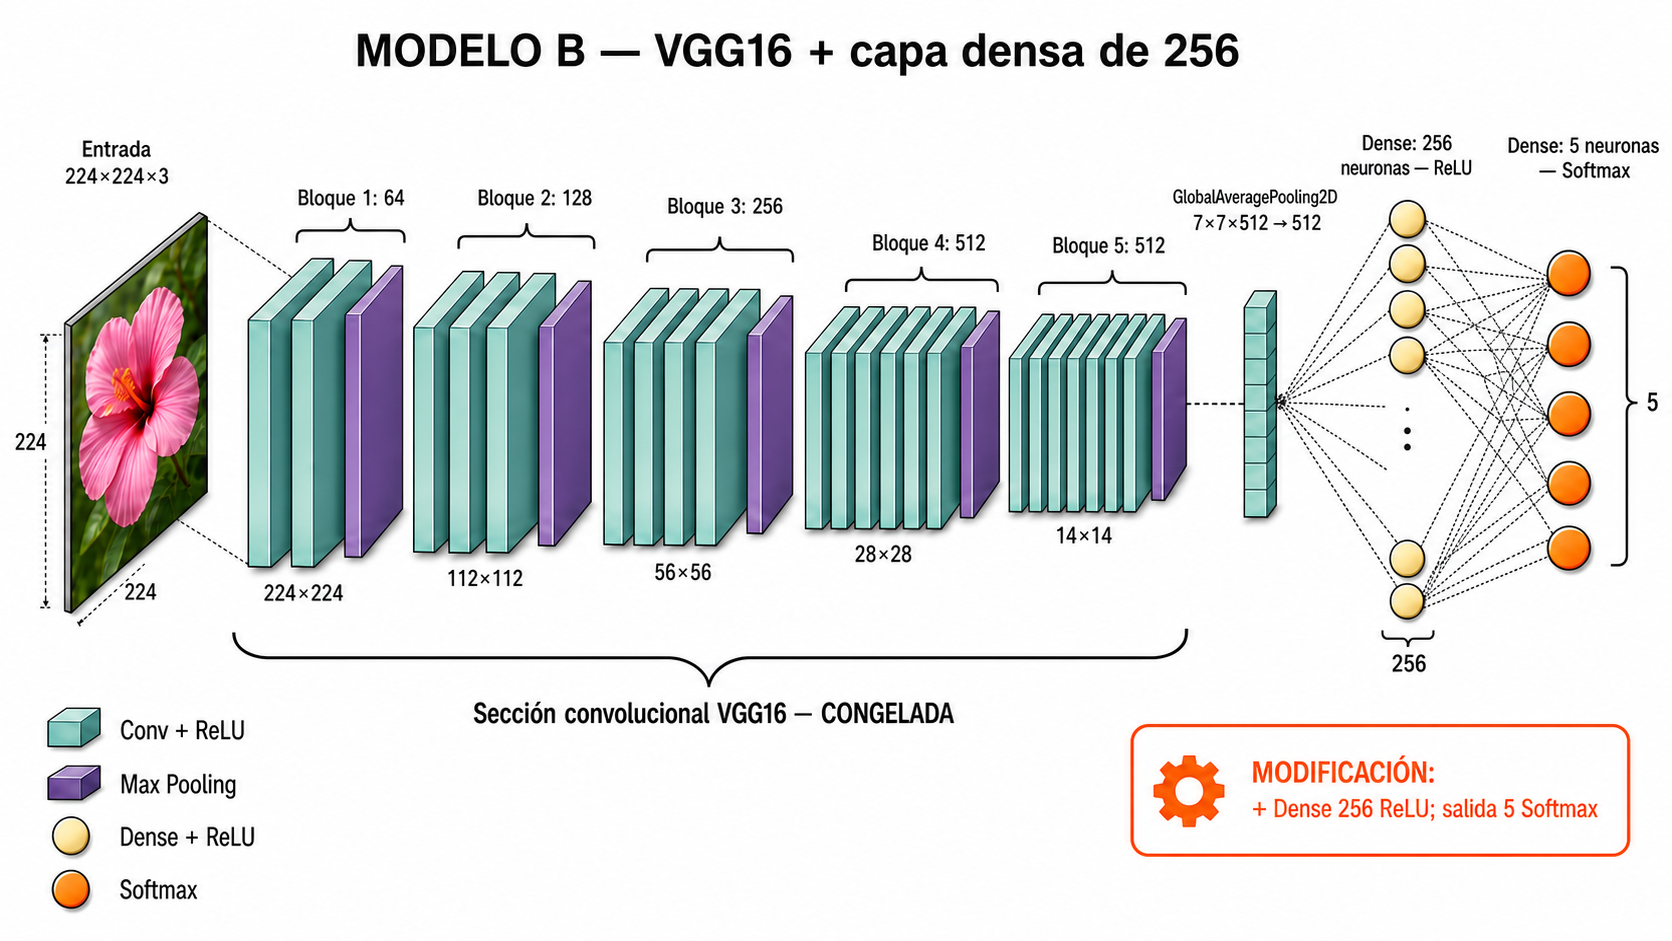
\includegraphics[width=.94\textwidth,height=.68\textheight,keepaspectratio]{arquitectura_modelo_B_visual.png}
\vspace{.08cm}
\begin{beamercolorbox}[rounded=true,sep=.35em,center,wd=.94\textwidth]{block body}
\scriptsize Después del promedio global, 256 unidades ReLU recombinan las características antes de producir las cinco probabilidades.
\end{beamercolorbox}
\end{frame}

% 8 — 0:40
\begin{frame}{Modelo C: cabezal profundo regularizado}
\centering
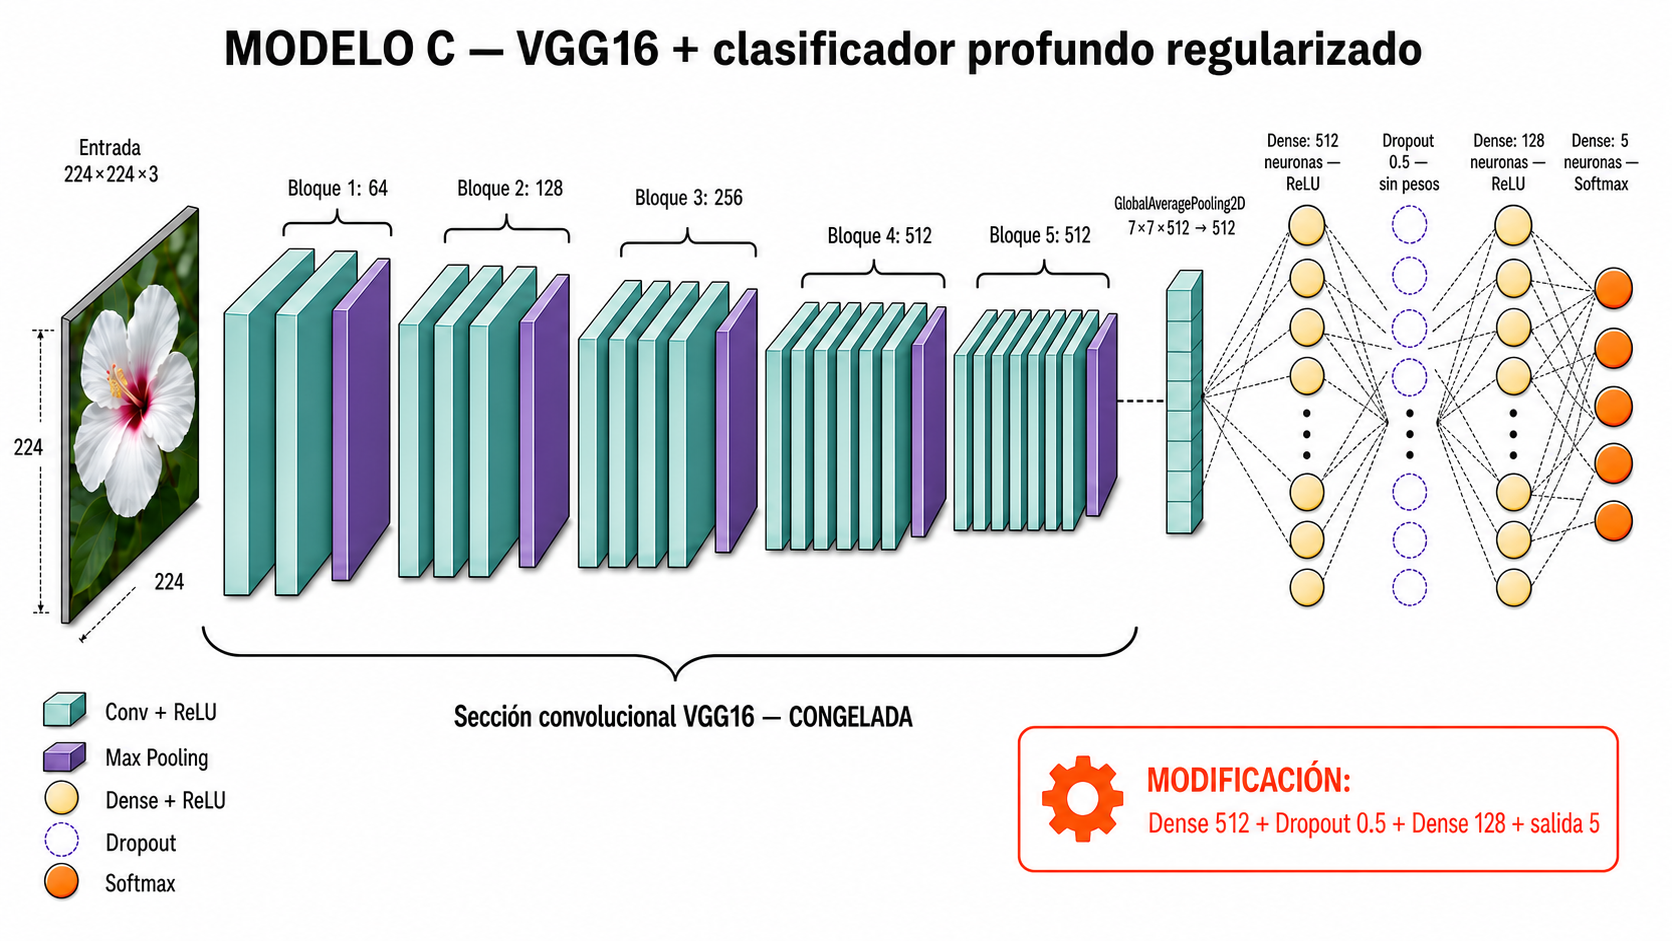
\includegraphics[width=.94\textwidth,height=.68\textheight,keepaspectratio]{arquitectura_modelo_C_visual.png}
\vspace{.08cm}
\begin{beamercolorbox}[rounded=true,sep=.35em,center,wd=.94\textwidth]{block body}
\scriptsize El cabezal utiliza 512 unidades, \texttt{Dropout(0.5)} y 128 unidades antes de la salida; es la variante de mayor capacidad.
\end{beamercolorbox}
\end{frame}

% 9 — 1:10
\begin{frame}{Protocolo reproducible y justo}
\begin{columns}[T,onlytextwidth]
\column{.48\textwidth}
\begin{itemize}\setlength\itemsep{.5em}
\item Adam, tasa inicial $10^{-3}$
\item Lotes de 16; máximo 30 épocas
\item Aumentación solo en entrenamiento
\item \texttt{EarlyStopping} y mejor checkpoint
\item Prueba utilizada una vez al final
\end{itemize}
\column{.48\textwidth}
\begin{block}{Semilla 42}
Controla partición, inicialización, orden de lotes, aumentación y \texttt{Dropout}.
\end{block}
\vspace{.25cm}
\begin{alertblock}{Lo que no significa}
No mejora el modelo ni elimina todo el no determinismo. Una sola semilla no mide variabilidad estadística.
\end{alertblock}
\end{columns}
\end{frame}

% 7 — 1:15
\begin{frame}{Cómo evalué los modelos}
\begin{columns}[T,onlytextwidth]
\column{.45\textwidth}
\dato{F1 macro}{criterio principal: mismo peso para cada clase}
\vspace{.35cm}
\begin{itemize}\setlength\itemsep{.42em}
\item Accuracy: aciertos totales
\item Precision: calidad de las predicciones positivas
\item Recall: ejemplos reales encontrados
\item F1: equilibrio entre Precision y Recall
\end{itemize}
\column{.51\textwidth}
\begin{block}{Sobreajuste}
El entrenamiento mejora, pero validación o prueba empeoran: el modelo aprendió particularidades que no generalizan.
\end{block}
\vspace{.25cm}
\centering
\begin{tikzpicture}[x=1cm,y=1cm]
\draw[->,Azul] (0,0)--(4.2,0) node[right,font=\scriptsize]{épocas};
\draw[->,Azul] (0,0)--(0,2.4) node[above,font=\scriptsize]{desempeño};
\draw[thick,Verde] plot[smooth] coordinates {(0,.3)(1,1.1)(2,1.7)(3,2)(4,2.18)};
\draw[thick,Rojo] plot[smooth] coordinates {(0,.3)(1,1)(2,1.45)(3,1.42)(4,1.2)};
\node[Verde,font=\scriptsize] at (3.5,2.28) {entrenamiento};
\node[Rojo,font=\scriptsize] at (3.6,1.05) {validación};
\end{tikzpicture}
\end{columns}
\end{frame}

% 8 — 1:30
\begin{frame}{Resultado principal: más parámetros no fue mejor}
\begin{columns}[T,onlytextwidth]
\column{.56\textwidth}
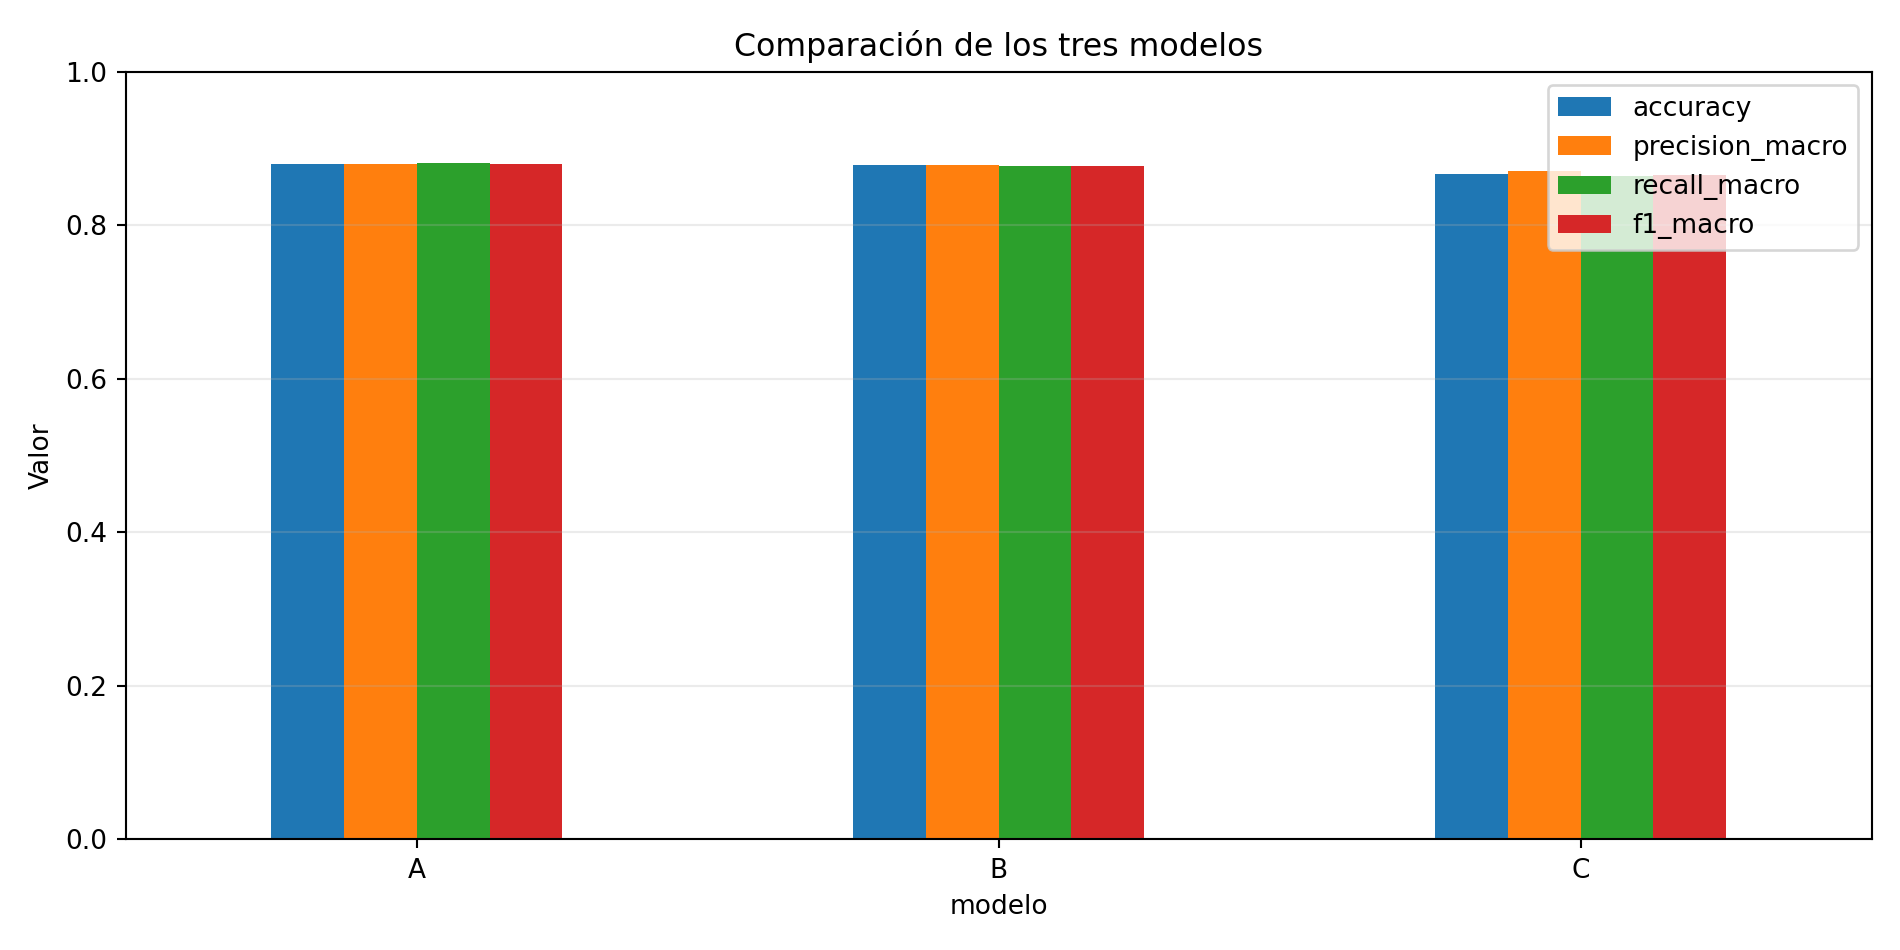
\includegraphics[width=\linewidth,height=.68\textheight,keepaspectratio]{comparacion_modelos.png}
\column{.41\textwidth}
\small
\begin{tabular}{@{}lrr@{}}
\toprule
& \textbf{Accuracy} & \textbf{F1 macro}\\
\midrule
\color{Verde}\bfseries A & \textbf{0.8802} & \textbf{0.8799}\\
B & 0.8784 & 0.8775\\
C & 0.8675 & 0.8652\\
\bottomrule
\end{tabular}
\vspace{.45cm}
\begin{block}{Modelo seleccionado: A}
Mejor F1 macro y Accuracy, menor brecha validación--prueba (0.0219) y solo 2,565 parámetros entrenables.
\end{block}
\vspace{.2cm}
{\scriptsize La ventaja de A sobre B es pequeña: $\Delta F1\approx0.0025$.}
\end{columns}
\end{frame}

% 9 — 0:50
\begin{frame}{Curvas de aprendizaje del Modelo A}
\centering
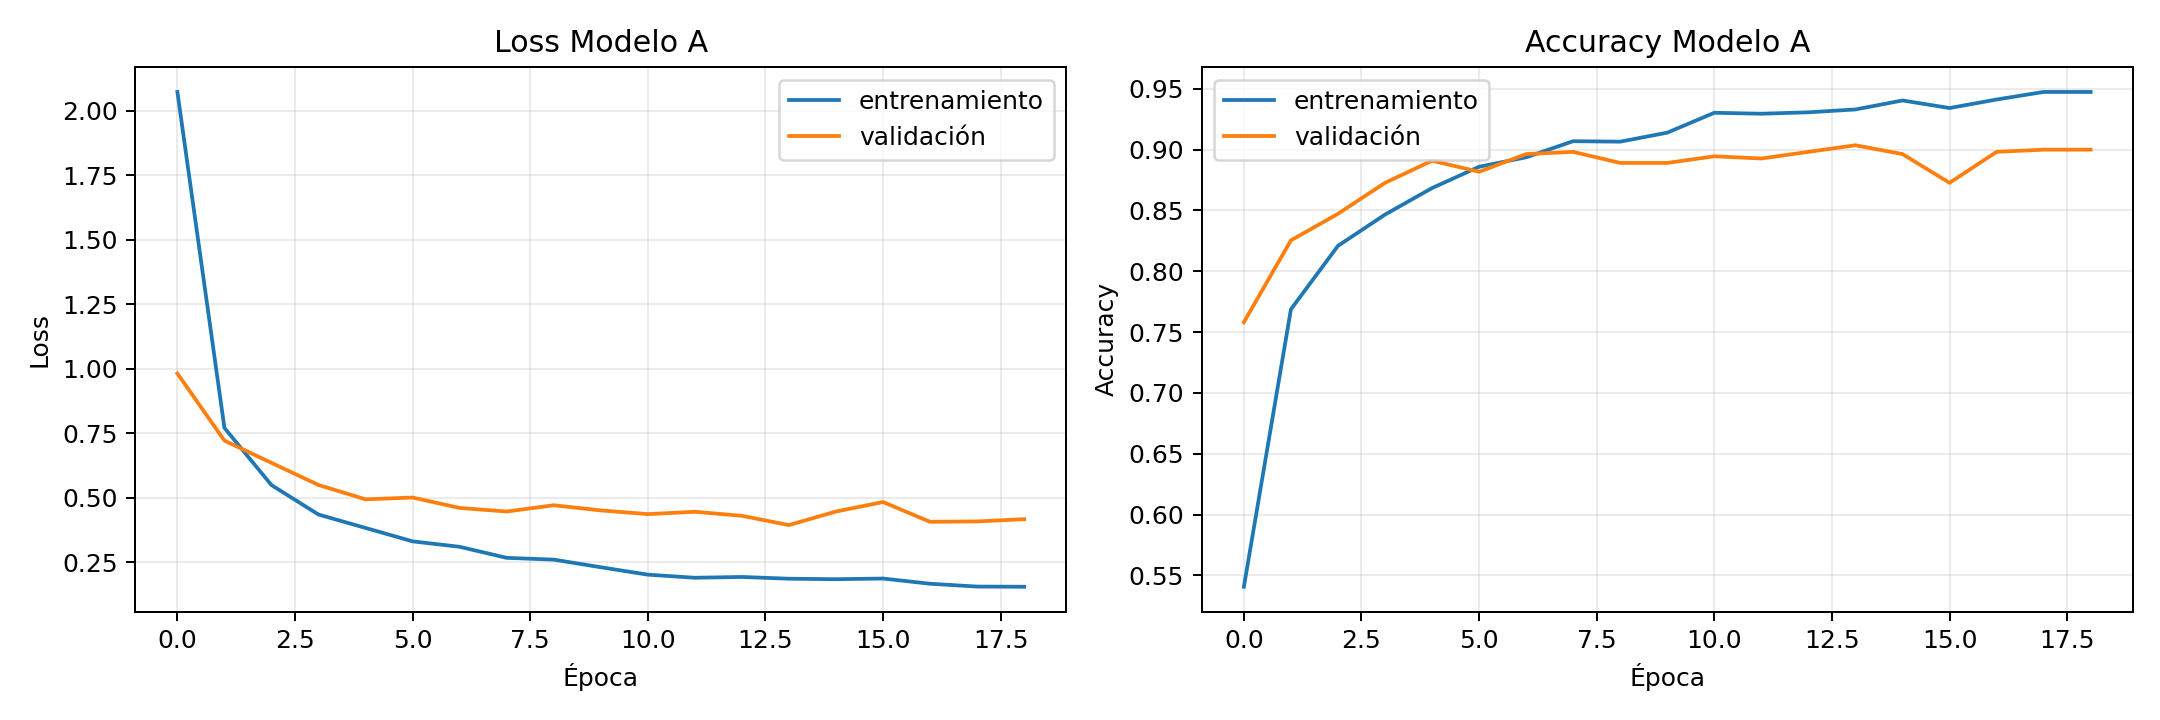
\includegraphics[width=.88\textwidth,height=.66\textheight,keepaspectratio]{curvas_modelo_A.png}
\vspace{.15cm}
\begin{beamercolorbox}[rounded=true,sep=.4em,center,wd=.88\textwidth]{block body}
\scriptsize Izquierda: \textbf{Loss} (menor es mejor). Derecha: \textbf{Accuracy} (mayor es mejor). Azul: entrenamiento; naranja: validación. Mejor checkpoint: época 14.
\end{beamercolorbox}
\end{frame}

% 10 — 0:50
\begin{frame}{Curvas de aprendizaje del Modelo B}
\centering
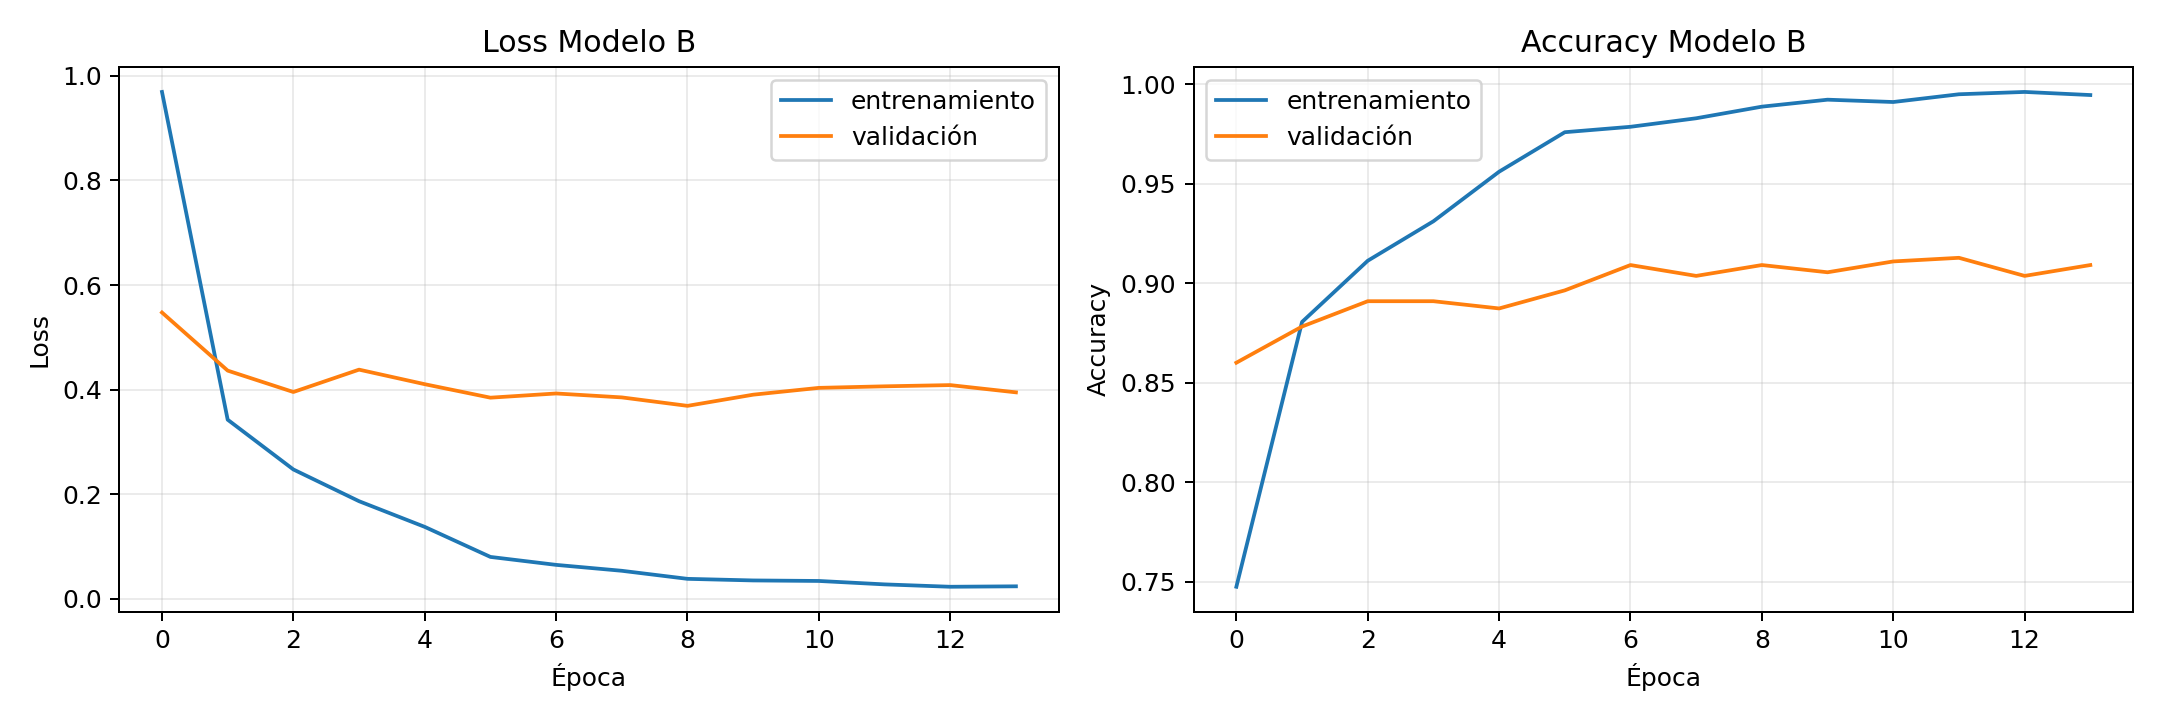
\includegraphics[width=.88\textwidth,height=.66\textheight,keepaspectratio]{curvas_modelo_B.png}
\vspace{.15cm}
\begin{beamercolorbox}[rounded=true,sep=.4em,center,wd=.88\textwidth]{block body}
\scriptsize Izquierda: \textbf{Loss}; derecha: \textbf{Accuracy}. La separación entre entrenamiento y validación indica menor generalización. Mejor checkpoint: época 9.
\end{beamercolorbox}
\end{frame}

% 11 — 0:50
\begin{frame}{Curvas de aprendizaje del Modelo C}
\centering
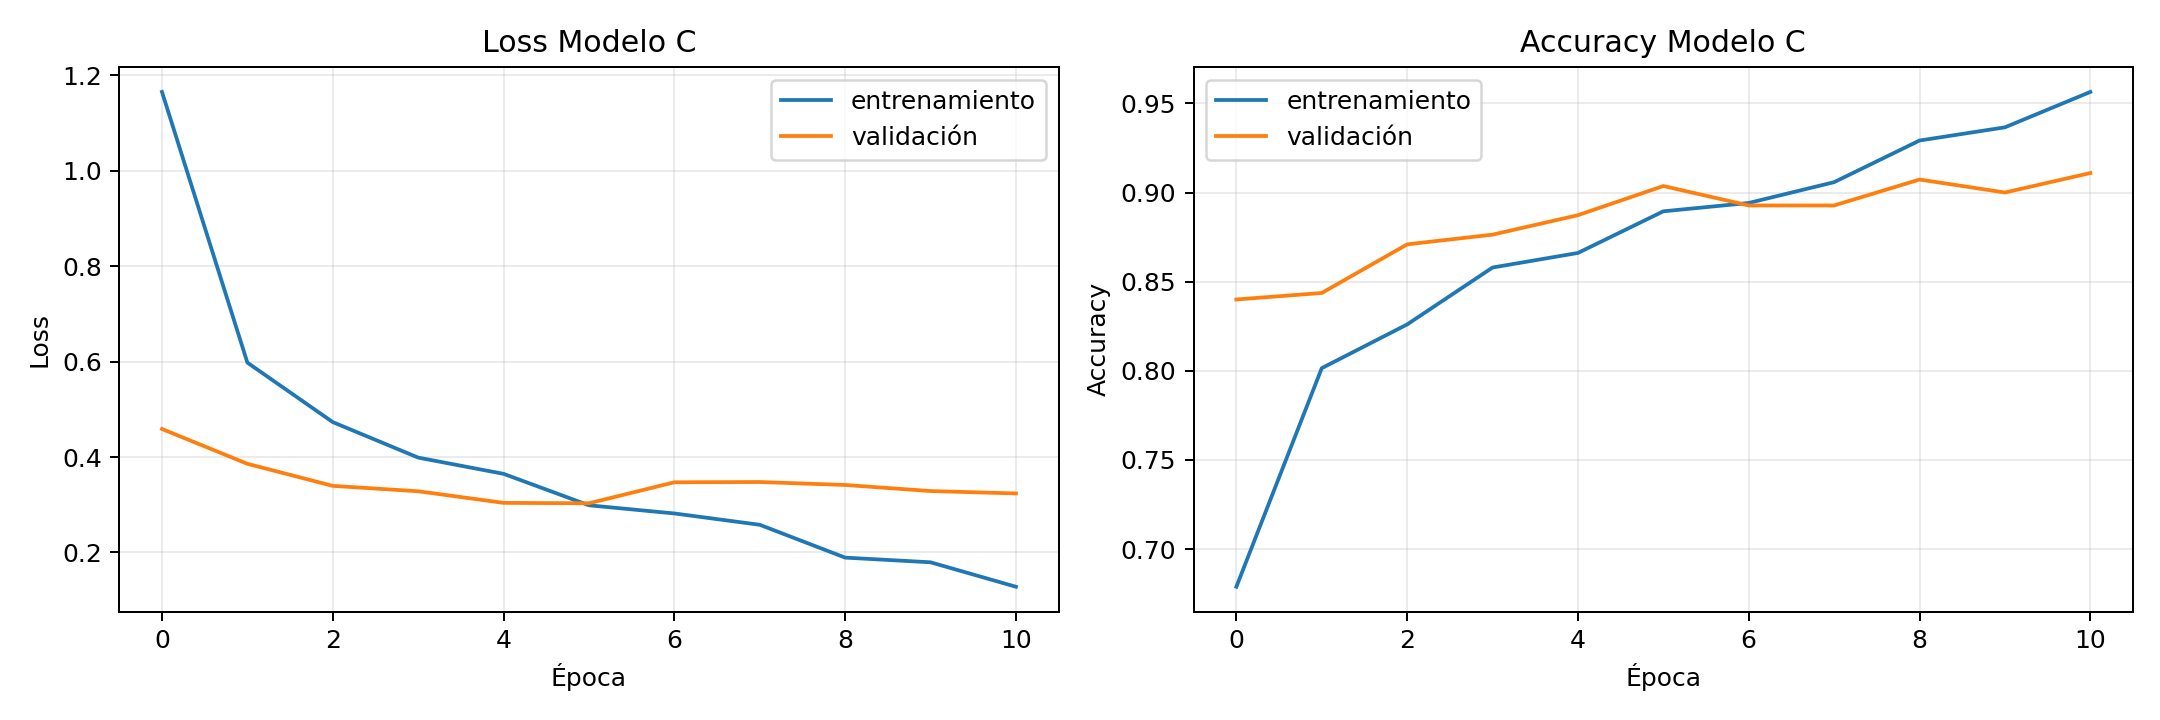
\includegraphics[width=.88\textwidth,height=.66\textheight,keepaspectratio]{curvas_modelo_C.png}
\vspace{.15cm}
\begin{beamercolorbox}[rounded=true,sep=.4em,center,wd=.88\textwidth]{block body}
\scriptsize Azul: entrenamiento; naranja: validación. Una brecha creciente puede indicar sobreajuste. Mejor checkpoint: época 6; \texttt{Dropout} no garantiza una mejora.
\end{beamercolorbox}
\end{frame}

% 12 — 1:20
\begin{frame}{?`Dónde acierta y dónde se confunde el Modelo A?}
\begin{columns}[T,onlytextwidth]
\column{.60\textwidth}
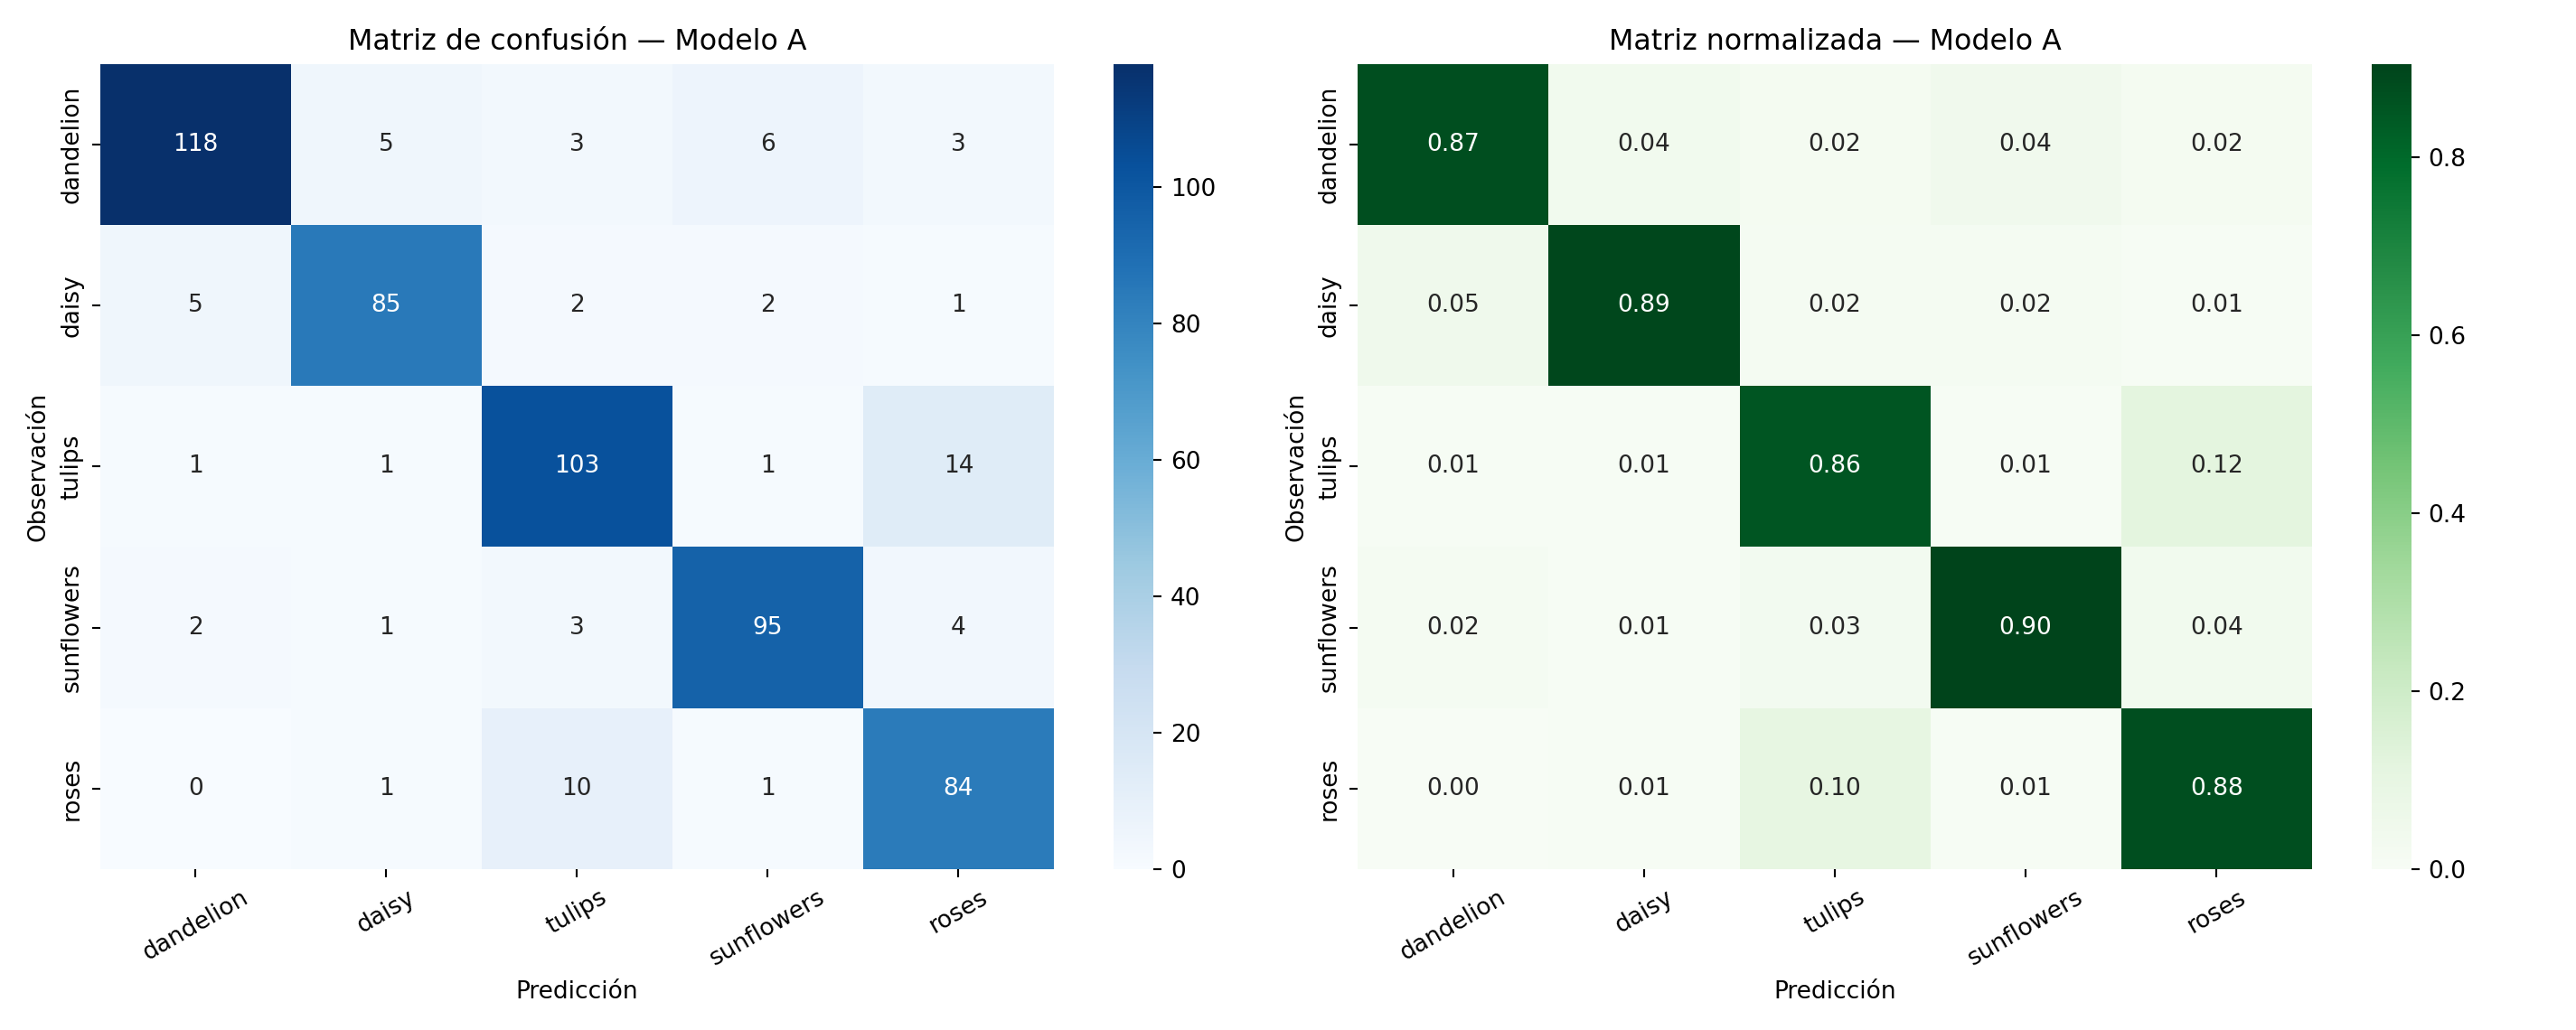
\includegraphics[width=\linewidth,height=.59\textheight,keepaspectratio]{matrices_confusion_modelo_A.png}
\column{.37\textwidth}
\dato{0.9048}{mejor F1: sunflowers}
\vspace{.15cm}
\dato{0.8317}{menor F1: roses}
\vspace{.15cm}
\begin{block}{Confusión dominante}
\centering tulips $\leftrightarrow$ roses
\end{block}
\vspace{.1cm}
{\scriptsize El error más frecuente aparece entre tulips y roses.}
\end{columns}
\centering{\tiny Filas = clase real; columnas = predicción. La diagonal son aciertos. Izquierda: cantidades; derecha: proporciones por clase.}
\end{frame}

% 13 — 0:50
\begin{frame}{Matriz de confusión del Modelo B}
\begin{columns}[T,onlytextwidth]
\column{.67\textwidth}
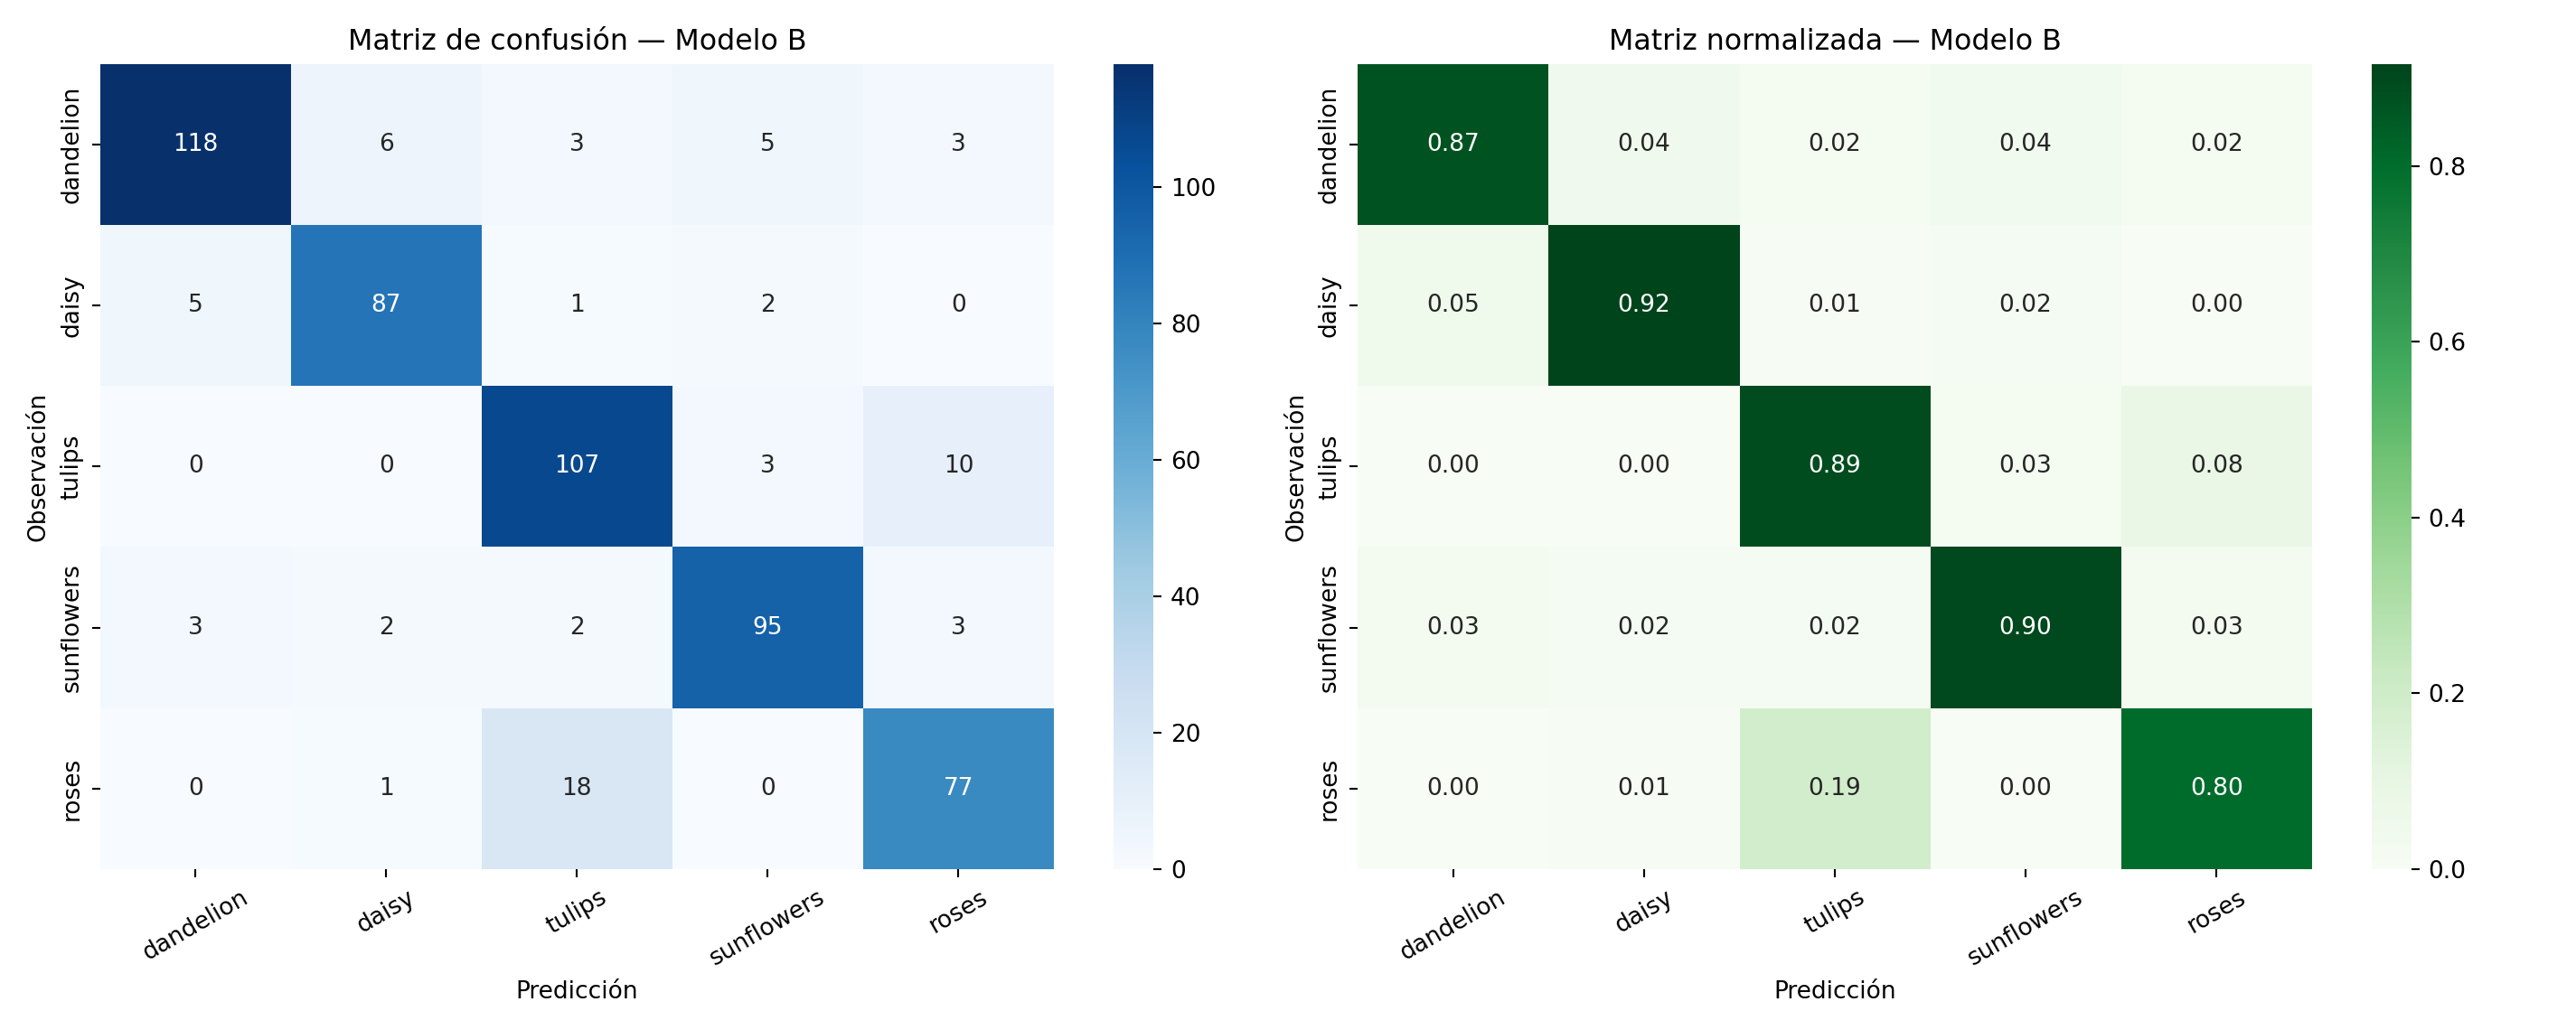
\includegraphics[width=\linewidth,height=.70\textheight,keepaspectratio]{matrices_confusion_modelo_B.png}
\column{.30\textwidth}
\begin{block}{Resultado global}
\centering\Large\bfseries F1 macro\\[.15cm]0.8775
\end{block}
\vspace{.25cm}
{\small B queda muy cerca de A, pero utiliza 132,613 parámetros entrenables y presenta una brecha validación--prueba de 0.0308.}
\end{columns}
\vspace{.12cm}
\centering{\scriptsize Diagonal = aciertos; celdas externas = confusiones. La matriz derecha normaliza cada fila para comparar clases.}
\end{frame}

% 14 — 0:50
\begin{frame}{Matriz de confusión del Modelo C}
\begin{columns}[T,onlytextwidth]
\column{.67\textwidth}
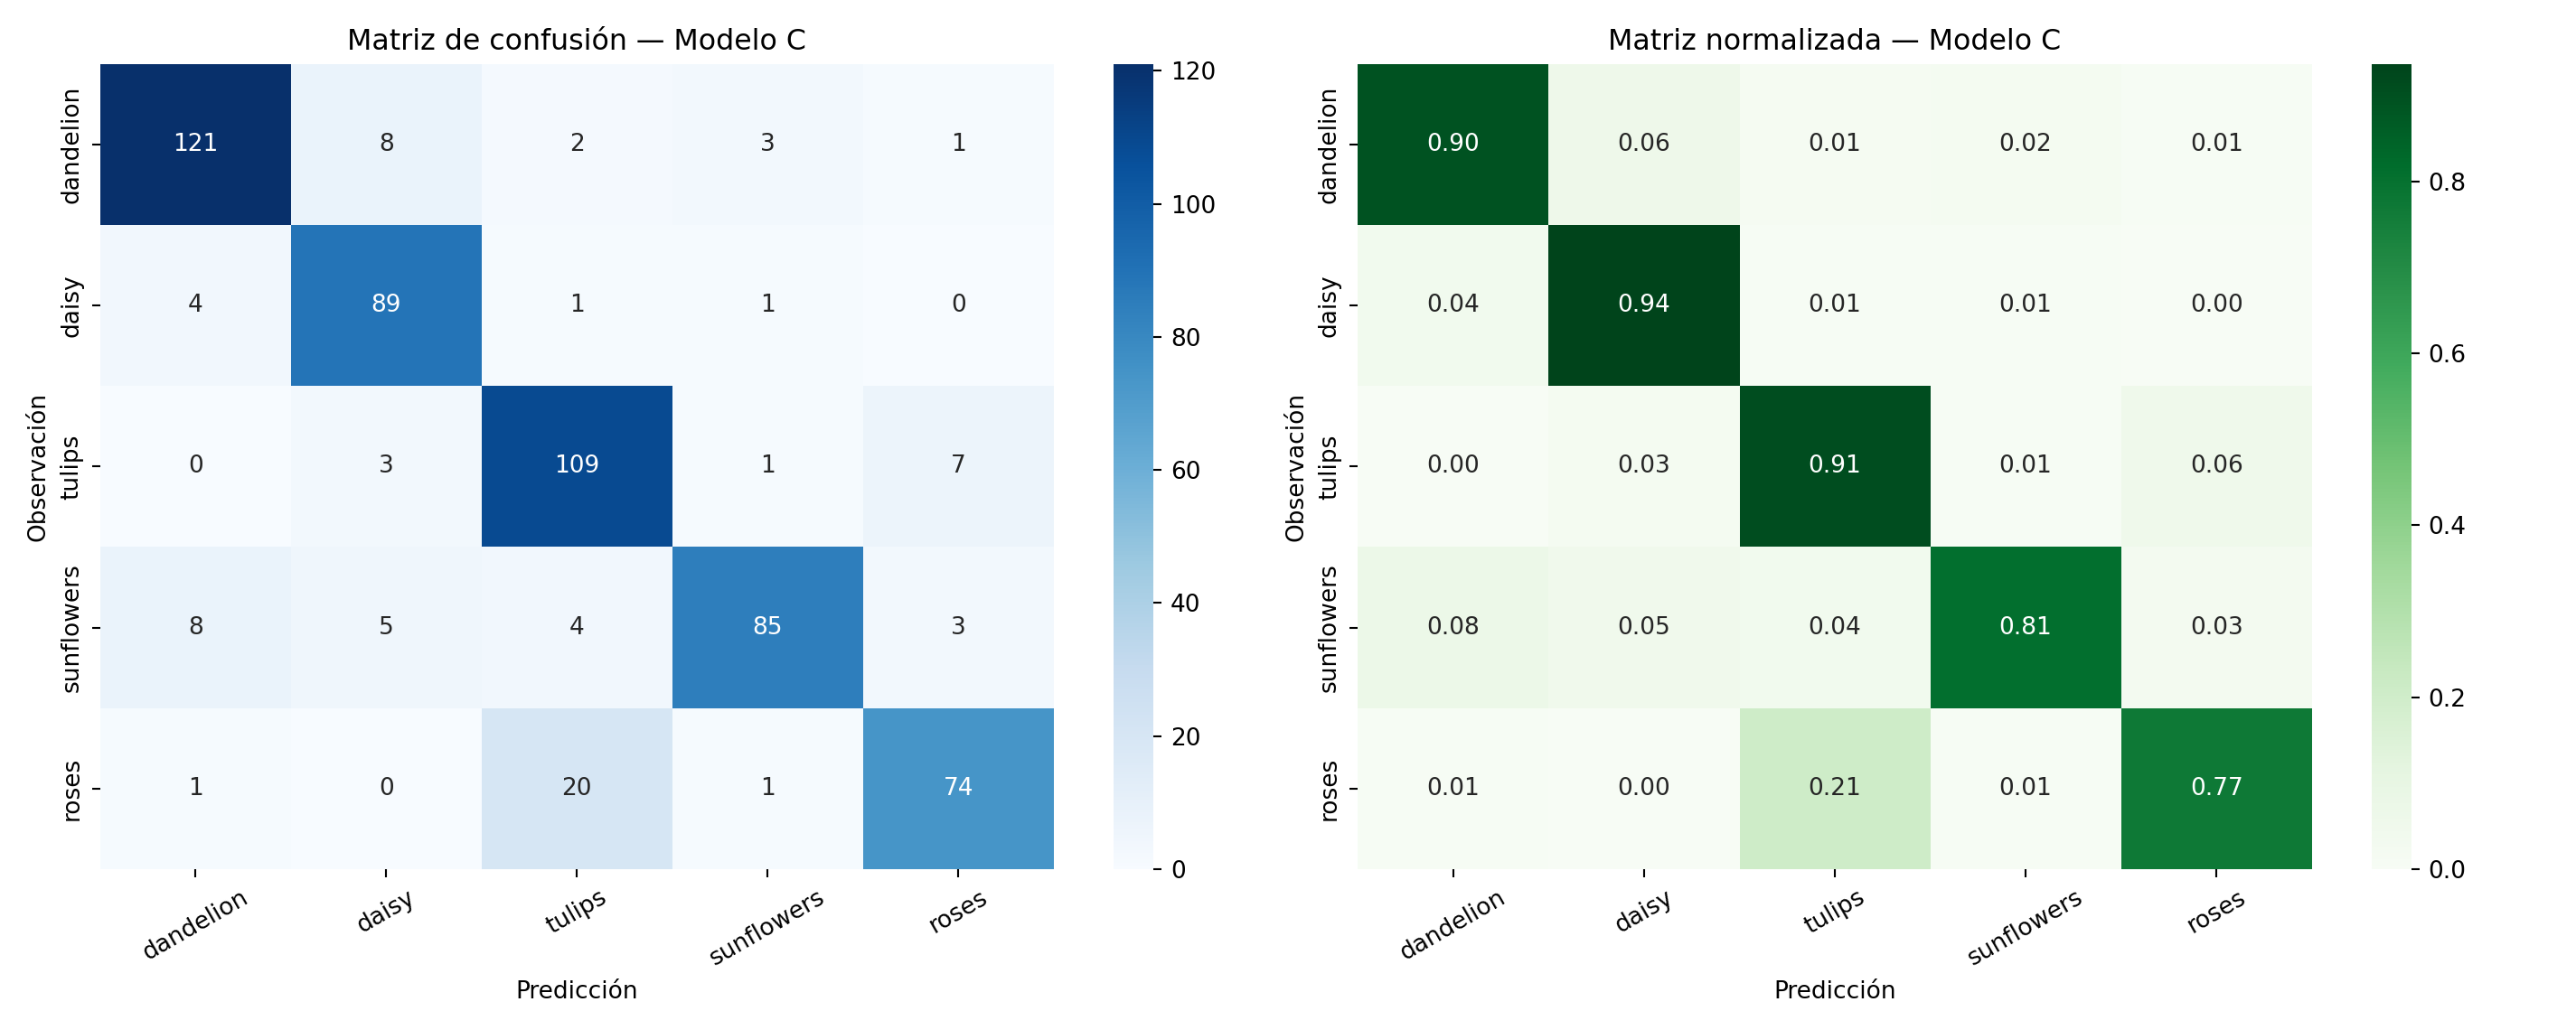
\includegraphics[width=\linewidth,height=.70\textheight,keepaspectratio]{matrices_confusion_modelo_C.png}
\column{.30\textwidth}
\begin{block}{Resultado global}
\centering\Large\bfseries F1 macro\\[.15cm]0.8652
\end{block}
\vspace{.25cm}
{\small C incorpora mayor capacidad y \texttt{Dropout}, pero alcanza el menor F1 y la mayor brecha validación--prueba: 0.0367.}
\end{columns}
\vspace{.12cm}
\centering{\scriptsize Filas = clase real; columnas = predicción. La matriz normalizada muestra la proporción de cada clase asignada a cada salida.}
\end{frame}

% 15 — 1:20
\begin{frame}{Conclusiones, límites y siguiente paso}
\begin{columns}[T,onlytextwidth]
\column{.48\textwidth}
\begin{block}{Lo que encontré}
\begin{itemize}\setlength\itemsep{.45em}
\item VGG16 congelada ya aporta características útiles.
\item A ofreció el mejor equilibrio entre desempeño y complejidad.
\item Más capas aumentaron capacidad, no información.
\item \textbf{La complejidad debe justificarse con evidencia.}
\end{itemize}
\end{block}
\column{.48\textwidth}
\begin{alertblock}{Límites}
\begin{itemize}\setlength\itemsep{.38em}
\item 3,670 imágenes y una sola semilla
\item Sin búsqueda exhaustiva de hiperparámetros
\item Sin \emph{fine-tuning} de VGG16
\item Diferencia A--B pequeña, sin prueba de significancia
\end{itemize}
\end{alertblock}
\vspace{.2cm}
\begin{block}{Trabajo futuro}
Repetir con varias semillas y evaluar \emph{fine-tuning} parcial.
\end{block}
\end{columns}
\end{frame}

% 16 — 0:20
\begin{frame}[plain]
\begin{tikzpicture}[remember picture,overlay]
\node[inner sep=0pt] at (current page.center) {
\includegraphics[width=\paperwidth,height=\paperheight]{meme_modelo_a.png}};
\node[rounded corners=5pt,fill=AzulNoche,
      inner xsep=13pt,inner ysep=7pt,text=white,font=\LARGE\bfseries,
      xshift=.6cm,yshift=.35cm] at (current page.center) {?`Preguntas?};
\end{tikzpicture}
\end{frame}

\end{document}
